\documentclass[final]{template}
\usepackage[utf8]{vietnam}
\usepackage{placeins}
\usepackage{amsfonts}
\usepackage{textcomp}
\usepackage{dblfloatfix}
\usepackage{lineno}
\usepackage{amssymb}
\usepackage{tabularx,booktabs}
\usepackage{longtable, lipsum}
\usepackage{amsmath}
\usepackage{mathtools}
\usepackage{graphicx}
\usepackage{lscape}
\usepackage{caption}
\usepackage{lmodern}
\usepackage{hyperref}
\usepackage[sorting=nyt]{biblatex}
\usepackage{mathtools}
\usepackage{lipsum}
\usepackage{fancyhdr}
\usepackage{titlesec}
\usepackage{makecell}
\usepackage{listings}
\usepackage{subcaption}
\usepackage{adjustbox}
\usepackage[vietnamese,english]{babel}
\usepackage{multirow}
\usepackage{longtable}
\usepackage{rotating}

% Define color and column type
\definecolor{dkgreen}{rgb}{0,0.6,0}
\definecolor{gray}{rgb}{0.5,0.5,0.5}
\definecolor{mauve}{rgb}{0.58,0,0.82}
\newcolumntype{C}[1]{>{\centering\arraybackslash}m{#1}}

% Config reference source file
\addbibresource{ref.bib}

% Config figure path
\graphicspath{ {./graphics} }

% Config for math in quantum computin
\DeclarePairedDelimiter\bra{\langle}{\rvert}
\DeclarePairedDelimiter\ket{\lvert}{\rangle}
\DeclarePairedDelimiterX\braket[2]{\langle}{\rangle}{#1 \delimsize\vert#2}

% Config listings 
\lstset{
  frame=tb,
  aboveskip=3mm,
  belowskip=3mm,
  showstringspaces=false,
  columns=fullflexible,
  basicstyle={\small\ttfamily},
  numbers=left,
  numberstyle=\tiny\color{gray},
  keywordstyle=\color{blue},
  commentstyle=\color{dkgreen},
  stringstyle=\color{mauve},
  breaklines=true,
  postbreak=\mbox{\textcolor{red}{$\hookrightarrow$}\space},
  tabsize=3
}
% Config listings 
\lstset{
  frame=tb,
  aboveskip=3mm,
  belowskip=3mm,
  showstringspaces=false,
  columns=fullflexible,
  basicstyle={\small\ttfamily},
  numbers=left,
  numberstyle=\tiny\color{gray},
  keywordstyle=\color{blue},
  commentstyle=\color{dkgreen},
  stringstyle=\color{mauve},
  breaklines=true,
  postbreak=\mbox{\textcolor{red}{$\hookrightarrow$}\space},
  tabsize=3
}

% Config information thesis
% =========== Thay đổi thông tin tại phần này ===========
% \upperuniname{HỌC VIỆN CÔNG NGHỆ BƯU CHÍNH VIỄN THÔNG}
\uniname{HỌC VIỆN CÔNG NGHỆ BƯU CHÍNH VIỄN THÔNG}
\deptname{KHOA CÔNG NGHỆ THÔNG TIN}
\stumajor{KỸ SƯ NGÀNH HỆ THỐNG THÔNG TIN}
\title{MÔ HÌNH KẾT HỢP HÀNH VI ĐÁNH GIÁ VÀ BÌNH LUẬN CHO TƯ VẤN KHÁCH SẠN}
\supervisor{GIẢNG VIÊN HƯỚNG DẪN}
\supervisorname{TRẦN ĐÌNH QUẾ}
\stuname{VŨ QUANG SƠN }
\stunamewithid{VŨ QUANG SƠN - B17DCCN545}
\reporttime{NĂM 2021}
\reporttype{ĐỒ ÁN TỐT NGHIỆP ĐẠI HỌC}
\instruction{GIẢNG VIÊN HƯỚNG DẪN}
\reportplace{HÀ NỘI}

% =========== Hết phần thay đổi thông tin ===========

% Begin thesis

\begin{document}
\coverpage
\secondcoverpage

\frontmatter
\chapter*{\centering\Large{Lời cảm ơn}}
\addcontentsline{toc}{chapter}{Lời cảm ơn}

Lời đầu tiên, em xin gửi lời cảm ơn chân thành tới tất cả thầy cô đang giảng dạy
trong mái trường Học viện Công nghệ Bưu chính Viễn thông đã tận tình truyền đạt
những kinh nghiệm và kiến thức quý báu giúp em hoàn thành nhiệm vụ học tập trong
suốt khoảng thời gian hơn 4 năm là sinh viên của học viện. Em xin gửi lời biết ơn sâu
sắc đến thầy PGS.TS Trần Đình Quế, người đã tận tình hướng dẫn, chỉ bảo, định hướng
và nhắc nhở em trong suốt quá trình học tập cũng như hoàn thành đồ án này.


Cho con gửi lời cảm ơn chân thành đến bố mẹ, ông bà, anh chị em đã luôn động viên,
ủng hộ, cổ vũ và tạo điều kiện tốt nhất cho con trong suốt những năm tháng ngồi trên
ghế nhà trường.

Cuối cùng, cho tôi gửi lời cảm ơn đến những người bạn, người anh, người chị của
tôi, những người luôn chia sẻ, động viên, giúp đỡ và ở bên tôi mỗi khi tôi gặp khó khăn
nhất!

Em xin chân thành cảm ơn!

\begin{flushright}
\textit {Hà Nội, ngày 10 tháng 12 năm 2021} \\
\textit{Sinh viên thực hiện} \\
\textit {Vũ Quang Sơn}
\end{flushright}


\tableofcontents
\clearpage
\listoffigures
\clearpage
\listoftables
\clearpage
\lstlistoflistings
\chapter*{\centering\Large{Danh mục từ viết tắt và tạm dịch}}
\addcontentsline{toc}{chapter}{Danh mục từ viết tắt và tạm dịch}


\begin{table}[htbp]
\centering
\begin{tabular}{|>{\centering\arraybackslash}p{.1\textwidth}|p{.35\textwidth}|p{.35\textwidth}|}
        \hline
        \multicolumn{1}{|c|}{\textbf{\begin{tabular}[c]{@{}c@{}}Từ viết\\ tắt\end{tabular}}} & \textbf{Tiếng Anh} & \textbf{Tạm dịch}\\
        \hline
        CF &  Collaborative Filtering & Lọc cộng tác  \\
        SVD &  Singular Value Decomposition & Phân tích giá trị đơn vị đặc biệt  \\
        PCA &  Principal Component Analysis & Phân tích thành phần chính  \\
        MBCF & Memory-based Collaborative Filtering & Lọc cộng tác dựa trên bộ nhớ \\
        UBCF & User-based Collaborative Filtering & Lọc cộng tác dựa trên người dùng \\
        IBCF & Item-based Collaborative Filtering & Lọc cộng tác dựa trên sản phẩm \\
        KNN & K-Nearest Neighbors & K láng giềng gần nhất \\
        \hline
\end{tabular}
\label{tab:example}
\end{table}
\chapter*{\centering\Large{Danh mục từ tạm dịch}}
\addcontentsline{toc}{chapter}{Danh mục từ tạm dịch}
\begin{tabular}{| p{.4\textwidth} |p{.4\textwidth} |}
\hline
        Machine Learning &  Học máy\\
        \hline
        Deep Learning & Học sâu \\
        \hline
        Reinforcement learning & Học tăng cường \\
        \hline
        Federated Learning & Học liên kết\\
        \hline
\end{tabular} \\



\clearpage

% Begin main thesis, start page numbering
\counterwithin{equation}{chapter}
\counterwithin{table}{chapter}
\counterwithin{figure}{chapter}
\setcounter{secnumdepth}{3}
\mainmatter

% Config page header
\fancyhf{}
\fancyfoot[C]{\thepage}
% \chapter*{Tóm tắt khóa luận}
\chapter*{\centering\Large{Mở đầu}}
\addcontentsline{toc}{chapter}{Tóm tắt khóa luận}

Cuộc sống của con người ngày càng phát triển, các nhu cầu cá nhân như: giao lưu,
kết bạn, tiêu dùng, du lịch, … ngày tăng. Nhu cầu tiêu dùng ngày càng tăng, cùng với
sự phát triển của công nghệ thống tin, các hệ thống thương mại điện tử ra đời và ngày
càng lớn mạnh, tiêu biểu như: Facebook, Youtube, Tripadvisor, … Những trang thương
mại điện tử này hỗ trợ doanh nghiệp quảng bá sản phẩm tới tay người tiêu dùng nhanh
hơn so với bán hàng truyền thống. Tuy nhiên, khi người dùng được tiếp cận sản phẩm,
dịch vụ một cách nhanh chóng thì họ cũng phải đối mặt với vấn đề có quá nhiều sản
phẩm và dịch vụ và đâu thực sự là sản phẩm họ cần. Đây là tình trạng quá tải thông tin,
khi người dùng có quá nhiều lựa chọn. Tuy nhiên, đôi khi họ cũng phải đối mặt với tình
huống nghịch lý rằng có rất nhiều thông tin, nhưng thường rất khó để có thông tin phù
hợp \cite{edmunds2000problem}. Với hiện trạng nêu trên, nhu cầu cấp thiết đặt ra cần có các hệ thống tự động
hóa, hỗ trợ người dùng lọc thông tin cũng như cá nhân hóa đối với từng người dùng.

Hệ tư vấn ra đời nhằm giải quyết vấn đề quá tải thông tin từ người dùng, giúp họ
khám phá những sản phẩm khác nhau nằm trong sở thích của mình. Có rất nhiều trang
thương mại điện tử lớn sử dụng hệ tư vấn nhằm cải thiện doanh thu và tăng sự thân thiện
với người dùng, một trong số đó là Youtube. Youtube, ra đời vào tháng 2, 2005 với sự
phát triển nhanh chóng đã trở thành nền tảng chia sẻ video trực tuyến lớn nhất hiện nay
với hơn 1 tỷ lượt xem mỗi ngày từ hàng triệu người dùng và mỗi phút có hơn 24 giờ
thời lượng video được tải lên nền tảng này. Hệ tư vấn là một phần trong sự thành công
của Youtube khi đóng góp 60\% lượt bấm xem video từ trang chủ và các video được gợi
ý từ hệ thống có tỷ lệ bấm xem gấp 2 lần những video được nhiều người xem nhất và
được đánh giá cao nhất \cite{davidson2010youtube}.

Một trong các thuật toán tư vấn điển hình và phổ biến là lọc cộng tác và hoạt động
rất hiệu quả. Các hệ tư vấn truyền thống thường sử dụng dữ liệu điểm đánh giá để làm
cơ sở tư vấn. Tuy nhiên, theo \cite{isinkaye2015recommendation}, thuật toán này vẫn còn những vấn đề còn tồn tại như:
\begin{itemize}
    \item Vấn đề người dùng mới, sản phẩm mới (Cold Start)
    \item Vấn đề thưa thớt dữ liệu
\end{itemize}
Do thói quen lười đánh giá từ người dùng, gây ra những vấn đề trên ảnh hưởng tới độ
chính xác của hệ tư vấn lọc cộng tác.

Với sự bùng nổ của các trang thương mại điện tử, các hành vi bày tỏ quan điểm ngày
càng đa dạng và phong phú. Do đó, các phương pháp phân loại văn bản ngày càng được
cải thiện và trở nên chính xác hơn. Những dữ liệu văn bản này cũng mang ý nghĩa bày
tỏ quan điểm đối với sản phẩm.

Để hệ tư vấn có những đề xuất chính xác hơn cũng như tận dụng dữ liệu văn bản
cùng các kỹ thuật phân loại được phát triển, đồ án lựa chọn đề tài \textbf{"Mô hình kết hợp
hành vi đánh giá và bình luận cho tư vấn khách sạn"} với mục tiêu nghiên cứu lý thuyết về hệ tư vấn, các kỹ thuật tư vấn, tiền xử lý văn bản và phân loại văn bản về lĩnh
vực cụ thể là gợi ý các khách sạn trên các bộ dữ liệu thu thập được.

Đồ án được chia thành 4 chương với nội dung như sau:

\textbf{Chương 1: Tổng quan về hệ tư vấn} - Nội dung trong Chương 1 giới thiệu tổng quan về hệ tư vấn và các kỹ thuật lọc cộng
tác. Ngoài ra, Chương 1 còn trình bày ngắn gọn các vấn đề còn tồn tại của hệ tư vấn lọc
cộng tác.

\textbf{Chương 2: Tư vấn dựa trên mô hình kết hợp} - Trong chương này, đồ án trình bày về mô hình kết hợp giữa hành vi đánh giá và hành
vi bình luận và cách ứng dụng mô hình kết hợp vào hệ tư vấn lọc cộng tác. Ngoài ra, nội
dung Chương 2 còn trình bày về các kỹ thuật tiền xử lý dữ liệu văn bản cùng với 3 kỹ
thuật phân loại văn bản: Naïve Bayes, Logistic Regression, SVM.

\textbf{Chương 3: Thử nghiệm và đánh giá} - Chương 3 tập trung trình bày về bộ dữ liệu được thử nghiệm, phương pháp thực
nghiệm, bộ dữ liệu được sử dụng và kết quả thực nghiệm và đánh giá.

\if @twoside
  \fancyhead[EL,OR]{\bfseries\nouppercase\rightmark}
\else
  \fancyhead[R]{\bfseries\nouppercase\rightmark}
\fi


\chapter{Đặt vấn đề}
\label{chap1}

Trong Chương \ref{chap1}, đồ án trình bày một cách tổng quan về hệ tư vấn. Ngoài ra, vai trò,
lợi ích của hệ tư vấn đối với thương mại điện tử cũng được trình bày trong chương này.
Nội dung của Chương 1 được phân chia như sau:
\chapter{Cơ sở lý thuyết}
\label{chap2}

Hệ thống khuyến nghị là 1 công nghệ hỗ trợ đắc lực cho con người, 
giúp phân tích lượng dữ liệu khổng lồ được cung cấp bởi người dùng. 
Hệ thống dự đoán điểm của các sản phẩm, tạo 1 danh sách sắp xếp thứ các 
sản phẩm này cho mỗi người dùng, và giới thiệu tới người dùng những sản 
phẩm mà họ có thể thích. Nội dung trong phần này trình bày tổng quan về 
hệ khuyến nghị, các mô hình thuật toán cùng với các kỹ thuật thuật khai 
phá dữ liệu trong hệ khuyến nghị hiện có.
\begin{figure}[htbp]
    \centering
    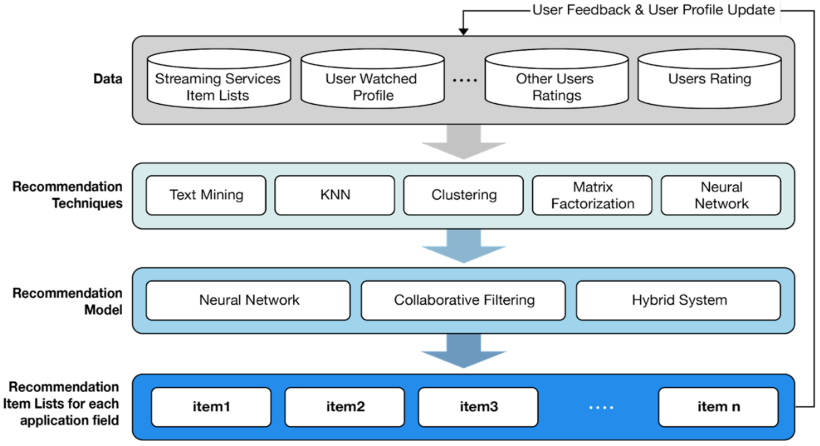
\includegraphics[width=1\textwidth]{imgs/chapter_2/tong-quan-htkn.png}
    \caption{Tổng quan hệ thống khuyến nghị}
    \label{tqhtkn}
\end{figure}
Hình \ref{tqhtkn} là tổng quan 
luồng hoạt động của 1 hệ khuyến nghị, gồm có các bước xử lý: (1) thu 
thập dữ liệu, (2) khai phá dữ liệu, (3) mô hình hóa dữ liệu, (4) và 
đưa ra gợi ý. Dữ liệu sử dụng trong hệ khuyến nghị có thể là các đánh 
giá, bình luận về sản phẩm, danh sách sản phẩm mà người dùng theo dõi, 
v.v. Các kỹ thuật khai phá dữ liệu truyền thống, có thể kể đến như: 
phân cụm, khai phá dữ liệu văn bản, KNN hay là học sâu, sử dụng mạng 
nơ-ron. Tiếp đó, các mô hình khuyến nghị sử dụng các đặc trưng đã 
được trích chọn để có thể mô hình hóa dữ liệu, từ đó đưa ra các khuyến 
nghị phù hợp tới người dùng.

Nội dung trong chương này tập trung giới thiệu và phân loại một cách tổng 
quát về các mô hình khuyến nghị hiện nay, có thể áp dụng vào bất kỳ 1 hệ thống khuyến
nghị nào.

\section{Phân loại mô hình khuyến nghị}
Các mô hình khuyến nghị có thể được chia thành 3 nhóm chính \cite{goyani2020review}:
\begin{itemize}
    \item \textbf{Lọc dựa trên nội dung}: Trong cách tiếp cận này, hệ thống sẽ thu thập các dữ
    liệu rõ ràng (điểm đánh giá sản phẩm) hoặc dữ liệu ngầm (bấm vào một đường
    dẫn) và tạo ra hồ sơ người dùng. Hệ thống sẽ thực hiện tư vấn những sản phẩm
    dựa trên những sản phẩm và hành vi liên quan tới hồ sơ người dùng. Do sở thích 
    của người dùng thường được chia thành vài nhóm cơ bản, việc chỉ sử dụng hồ sơ
    của 1 người dùng khiến hệ thống không tận dụng được thông tin từ những người
    dùng khác, từ đó hạn chế sự linh hoạt của hệ tư vấn.

    \item \textbf{Lọc cộng tác}: Không giống với lọc dựa trên nội dung, lọc cộng tác tìm kiếm
    những người dùng có sở thích tương tự nhau. Từ giả định những người dùng A
    có sở thích giống với người dùng B, hệ thống sẽ tiến hành tư vấn cho người dùng
    B những sản phẩm phù hợp người dùng A. Lọc cộng tác có 2 hướng tiếp cận: dựa
    trên bộ nhớ và dựa trên mô hình. Hướng tiếp cận dựa trên bộ nhớ tính toán độ
    tương tự giữa các người dùng từ đó thực hiện tư vấn. Nhược điểm của hướng tiếp
    cận này là sự tốn kém tài nguyên khi số lượng người dùng và sản phẩm tăng lên.
    Hướng tiếp cận dựa trên mô hình sử dụng các mô hình đã được huấn luyện thông
    qua các thuật toán học máy hoặc khai phá dữ liệu để thực hiện tư vấn.

    \item \textbf{Hệ tư vấn lai} Lọc dựa trên nội dung và lọc cộng tác đều có ưu điểm và nhược
    điểm riêng. Để giải quyết vấn đề này, hệ tư vấn lai được sinh ra, là sự kết hợp
    của 2 kỹ thuật trên.
\end{itemize}

Trong phần tiếp theo, đồ án sẽ tập trung vào việc trình bày mô hình 1 số lọc cộng
tác tiêu biểu.

\section{Lọc cộng tác}
Lọc cộng tác là một mô hình lọc thông tin, xây dựng 1 cơ sở dữ liệu sở thích người dùng 
thông qua dữ liệu tưởng tác giữa họ với sản phẩm để dự đoán các sản phẩm phù hợp với sở thích của họ, 
từ đó đưa ra các khuyến nghị về sản phẩm. Ý tưởng của mô hình lọc cộng tác là từ dữ liệu hành vi
tương tác giữa người dùng và sản phẩm, hệ thống sẽ tính toán mức độ tương đồng giữa các người dùng
hoặc giữa các sản phẩm, tạo cơ sở thực hiện khuyến nghị. Những người dùng có mức độ tương đồng cao
sẽ có xu hướng mua những sản phẩm giống nhau. Với mỗi cách tính độ tương đồng sẽ cho một mô hình lọc cộng tác 
khác nhau.

Các mô hình lọc cộng tác có thể được chia ra thông qua 2 hướng tiếp cận: lọc cộng tác dựa trên bộ nhớ và 
lọc cộng tác dựa trên mô hình. Hướng tiếp cận dựa trên bộ nhớ tính toán độ
tương tự giữa các người dùng từ đó thực hiện tư vấn. Nhược điểm của hướng tiếp
cận này là sự tốn kém tài nguyên khi số lượng người dùng và sản phẩm tăng lên. Ngoài ra, hệ 
thống cần tính toán tại thời điểm khuyến nghị, điều này sẽ ảnh hưởng tới thời gian đưa ra dự đoán.
Hướng tiếp cận dựa trên mô hình sử dụng các mô hình đã được huấn luyện thông
qua các thuật toán học máy hoặc khai phá dữ liệu để thực hiện tư vấn. Với hướng tiếp cận này, 
mô hình sẽ cần phải thực hiện huấn luyện trước, nhưng khi thực hiện khuyến nghị sẽ rất nhanh. 
Trong lọc cộng tác dựa trên bộ nhớ, ta có thể phân loại thành: 
lọc cộng tác dựa trên người dùng và lọc cộng tác dựa trên sản phẩm. Lọc cộng tác dựa trên người dùng là 
1 mô hình so sánh sự tương đồng giữa các người dùng thông qua dữ liệu tương tác của họ lên 
các sản phẩm, từ đó khuyến nghị các sản phẩm phù hợp. Lọc cộng tác dựa trên sản phẩm dự 
đoán bằng cách sử dụng độ tương đồng giữa sản phẩm và sản phẩm được chọn bởi người dùng 
thông qua 1 ma trận tương tác của người dùng và sản phẩm. Nói cách khác, lọc cộng tác dựa 
trên bộ nhớ sử dụng các kỹ thuật như: độ tương quan Pearson, độ tương quan cô-sin, KNN 
để tạo các nhóm có đặc tính giống nhau, từ đó khuyến nghị các sản phẩm tới người dùng trong 
nhóm. Do cách hoạt động dựa trên dữ liệu đánh giá, nên mô hình khó có thể hoạt động tốt 
khi không có đủ dữ liệu cần thiết. Để khắc phục vấn đề này, lọc cộng tác dựa trên mô hình 
đưa ra khuyến nghị nhờ sử dụng các thuật toán như: phân cụm, SVD hay PCA.

\subsection{Lọc cộng tác dựa trên bộ nhớ}

\begin{figure}[htbp]
    \centering
    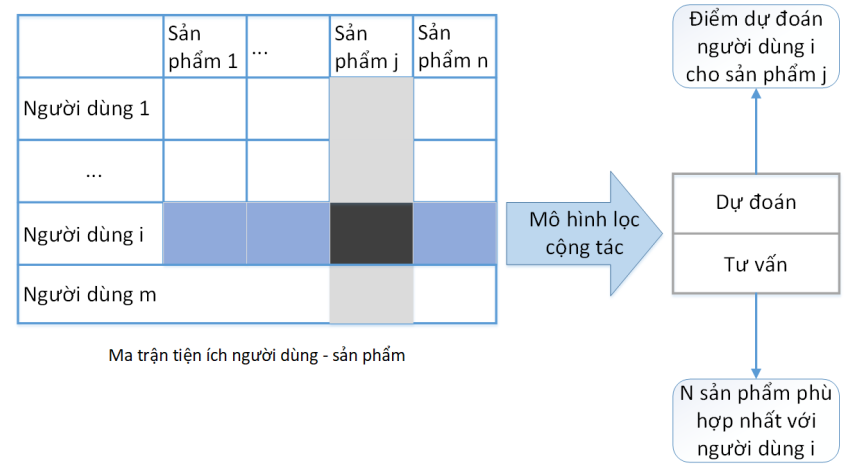
\includegraphics[width=1\textwidth]{imgs/chapter_2/loc-cong-tac.png}
    \caption{Mô hình thuật toán lọc cộng tác}
    \label{lct}
\end{figure}

\subsubsection{Lọc cộng tác dựa trên người dùng}
\chapter{Phương pháp giải quyết vấn đề}
\label{chap3}

\section{Hành vi người dùng trên mạng xã hội}

\subsection{Hành vi đánh giá}
Các hệ tư vấn thường được xây dựng từ:
\begin{itemize}
    \item Tập người dùng $W={w_1, w_2, ..., w_n}$
    \item Tập sản phẩm $X={x_1, x_2, ..., x_n}$
\end{itemize}
Hành vi đánh giá là hành động người dùng chấm điểm cho sản phẩm. Thông tin này
được lưu trữ và thường được sử dụng làm cơ sở cho hệ thống thực hiện tư vấn. Điểm
đánh giá từ người dùng $w_i$ cho sản phẩm $x_j$ được định nghĩa như sau:
\begin{equation}
    rating_{ij} = y, ~~~~~~ y \in {1, 2, ..., t}
\end{equation}
Trong đó, $t$ thường được chọn là 5 hoặc 10.

\subsection{Hành vi bình luận}
\label{hvbl}
Hành vi bình luận là hành động của người dùng khi diễn đạt suy nghĩ, quan điểm của
mình bằng văn bản. Người dùng thực hiện hành vi bình luận đối với sản phẩm thay vì
hành vi chấm điểm sẽ mô tả rõ hơn trải nghiệm, suy nghĩ của họ đối với sản phẩm. Mỗi
bình luận $comment_{ij}$ người dùng $w_i$ bày tỏ quan điểm đối với sản phẩm $x_j$. Bình luận
mang nhãn 0 nếu người dùng thích hoặc khen khách sạn. Ngược lại, bình luận mang
nhãn 1 nếu người dùng không thích hoặc chê khách sạn.
\begin{equation}
    comment_{ij} = \left\{
        \begin{array}{ c l }
            0 & \text{nếu $w_i$ thích $x_j$} \\ 
            1 & \text{nếu ngược lại}
        \end{array}
    \right.
\end{equation}

\subsection{Mô hình kết hợp hành vi đánh giá và hành vi bình luận}
Để sử dụng dữ liệu hành vi đánh giá và bình luận cùng lúc cho tư vấn khách sạn thì
cần có một phương pháp để kết hợp hai loại dữ liệu này. Như đã trình bày trong Phần
\ref{hvbl}: $rating_{ij}$: Điểm đánh giá từ người dùng $w_i$ cho sản phẩm $x_j$ và 
$comment_{ij}$: Bình luận bày tỏ quan điểm từ người dùng $w_i$ cho sản phẩm $x_j$.
Theo \cite{yang2022exploring}, các bình luận tiêu cực có ảnh hưởng không nhỏ tới quyết định 
mua hàng của người dùng. Tuy nhiên, nếu sản phẩm có nhiều phản hồi tích cực thì cũng làm tăng 
khả năng mua hàng của người dùng. Do đó, đồ án thực hiện kết hợp dựa trên ý tưởng:
\textbf{“Nếu khách sạn có bình luận tiêu cực thì điểm đánh giá dành cho khách sạn này cần
phải hạ xuống. Tuy nhiên, khách sạn có nhiều phản hồi tích cực thì điểm đánh giá
cũng cần được tăng lên”}. Điều này có nghĩa là, nếu khách sạn có nhiều phản hồi tích
cực thì các điểm đánh giá dành cho khách sạn này sẽ được thưởng thêm và ngược lại,
nếu khách sạn có nhiều bình luận phàn nàn thì điểm đánh giá sẽ bị trừ đi.

Với ý tưởng trên, điểm đánh giá dự đoán $rating_{ij}$ của người dùng $w_i$ với khách sạn
$x_j$ , tỷ lệ số bình luận tích cực $p\_rate_j$, tỷ lệ số bình luận tiêu cực 
$n\_rate_j$ của khách sạn $x_j$ sẽ là 3 thành phần quyết định tới điểm đánh giá cuối 
cùng dành cho  khách sạn. Coi điểm đánh giá cuối cùng là 100\%, $\alpha$ và $\beta$ là 2 trọng 
số tương ứng của $rating_{ij}$, $p\_rate_j$ và $n\_rate_j$ quyết định mức độ ảnh 
hưởng của 2 thành  phần này lên điểm đánh giá cuối cùng. Như vậy, điểm đánh giá cuối cùng 
của người dùng có thể  biểu diễn theo công thức:
\begin{equation}
    c\_rating(w_i, x_j) = \alpha \times rating_{ij} + \beta \times (p\_rate_j - n\_rate_j)
\end{equation}
Trong đó:
\begin{itemize}
    \item $c\_rating(w_i, x_j) \in [0; 5]$ là điểm đánh giá kết hợp, được sử dụng để làm dữ liệu thực
        hiện huấn luyện và đánh giá
    \item $rating_{ij} \in [0; 5]$ là điểm đánh giá được dự đoán thông qua thuật toán lọc 
        cộng tác, 
    \item $p\_rate_j \in [0; 1]$ là tỉ lệ số $comment_{ij}=0$ trong tổng số các 
        $comment_{ij}$ của sản phẩm $x_j$
    \item $n\_rate_j \in [0; 1]$ là tỉ lệ số $comment_{ij}=1$ trong tổng số các 
        $comment_{ij}$ của sản phẩm $x_j$
    \item Do $rating_{ij}$ nằm trong khoảng giá trị khác với $p\_rate_j$ và $n\_rate_j$ 
        vì vậy, trước khi thực hiện kết hợp, đồ án thực hiện chuyển $rating_{ij}$ về cùng 
        khoảng giá trị $[0;1]$ với $p\_rate_j$ và $n\_rate_j$ bằng cách 
        $rating_{ij}=\frac{rating_{ij}}{5}$
    \item Sau khi thực hiện tính toán, để đưa điểm đánh giá dự đoán về khoảng ban đầu,
        ta chỉ cần thực hiện $c\_rating(w_i, x_j) = c\_rating(w_i, x_j) \times 5$
\end{itemize}
\chapter{Thực nghiệm, kết quả, so sánh và đánh giá}
\label{chap4}

Thực nghiệm, kết quả, so sánh và đánh giá
\chapter{Kết luận}
\label{chap5}

Kết luận









\printbibliography[heading=bibintoc, title = {Tài liệu tham khảo}]
\end{document}